\documentclass[a4paper, 11pt]{article}
    \usepackage[utf8]{inputenc}
    \usepackage[english]{babel}
    \usepackage[breakable]{tcolorbox}
    \usepackage{indentfirst}
    \usepackage{graphicx}
    \usepackage{hyperref}
    \usepackage{color} 
    \usepackage{multirow}
    \usepackage{iftex}
    \ifPDFTeX
    	\usepackage[T1]{fontenc}
    	\usepackage{mathpazo}
    \else
    	\usepackage{fontspec}
    \fi
    \usepackage{caption}
    \DeclareCaptionFormat{nocaption}{}
    \captionsetup{format=nocaption,aboveskip=0pt,belowskip=0pt}

    \usepackage{float}
    \floatplacement{figure}{H} % forces figures to be placed at the correct location
    \usepackage{xcolor} % Allow colors to be defined
    \usepackage{enumerate} % Needed for markdown enumerations to work
    \usepackage{geometry} % Used to adjust the document margins
    \usepackage{amsmath} % Equations
    \usepackage{amssymb} % Equations
    \usepackage{textcomp} % defines textquotesingle


    \title{xklemr00\_knn\_project\_documentation}
    
    % Colors for the hyperref package
    \definecolor{urlcolor}{rgb}{0,.145,.698}
    \definecolor{linkcolor}{rgb}{.71,0.21,0.01}
    \definecolor{citecolor}{rgb}{.12,.54,.11}

    % Prevent overflowing lines due to hard-to-break entities
    \sloppy 
    % Setup hyperref package
    \hypersetup{
      breaklinks=true,  % so long urls are correctly broken across lines
      colorlinks=true,
      urlcolor=urlcolor,
      linkcolor=linkcolor,
      citecolor=citecolor,
      }
    % Slightly bigger margins than the latex defaults

    \geometry{verbose,tmargin=1in,bmargin=1in,lmargin=1in,rmargin=1in}
    
    
\begin{document}
    \begin{titlepage}
 \begin{center}
  {\Huge\textsc{Brno University of Technology\\[0.3em]
    \huge{Faculty of Information Technology}}}\\
  \vspace{\stretch{0.352}}
  {\Huge
  Generative image inpainting enhanced with edge focused WGAN-GP adversarial loss.}\\
  \vspace{\stretch{0.06}}
  {\Large Authors: Tomáš Beránek (xberan46), Richard Klem (xklemr00)}
  \vspace{\stretch{0.568}}
 \end{center}
 {\Large 
 \today 
 \hfill
}
\end{titlepage}

\newpage
\section{Abstract}
\label{section:abstract}
We improved the original model by adding third discriminator. The original solution uses local discriminator to calculate loss on the generated patch and global discriminator to calculate loss on the whole image. But very often, we can see clearly the edges of the patch, because there is no special attention to smooth transition between the generated patch and the rest of the image. We decided to provide a new discriminator, which will be focusing on the path with the near surroundings. This should help the generator to learn how to make a better transitions on the edges of the patch.

\section{Introduction}
\label{section:introduction}
For the time reasons, we made a decision to use just a subset of the Places2 dataset. We reduced our dataset to the 7 categories: \textit{army\_base}, \textit{badlands}, \textit{corn\_field},
\textit{forest\_path}, \textit{golf\_course}, \textit{hayfield} and \textit{mountain}. It makes 35 thousands of pictures in total. 3500 pictures were selected as testing/validation set.
The rest of 31 500 images serve as a training set.


\section{The original work and article}
\label{section:origin}
    \begin{figure}
        \centering
        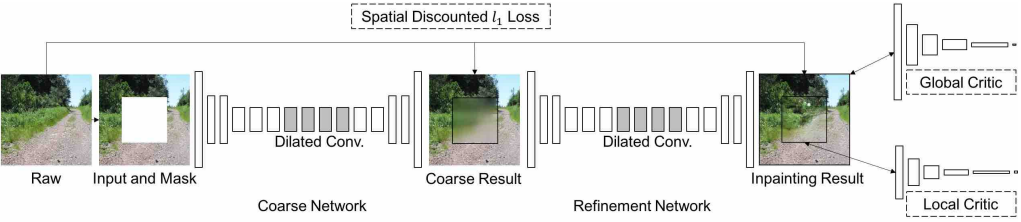
\includegraphics[width=0.95\linewidth]{documentation/img/original_arch.png}
    \end{figure}


\section{Edge focused discriminator}
\label{section:edgeDiscriminator}
    \begin{figure}
        \centering
        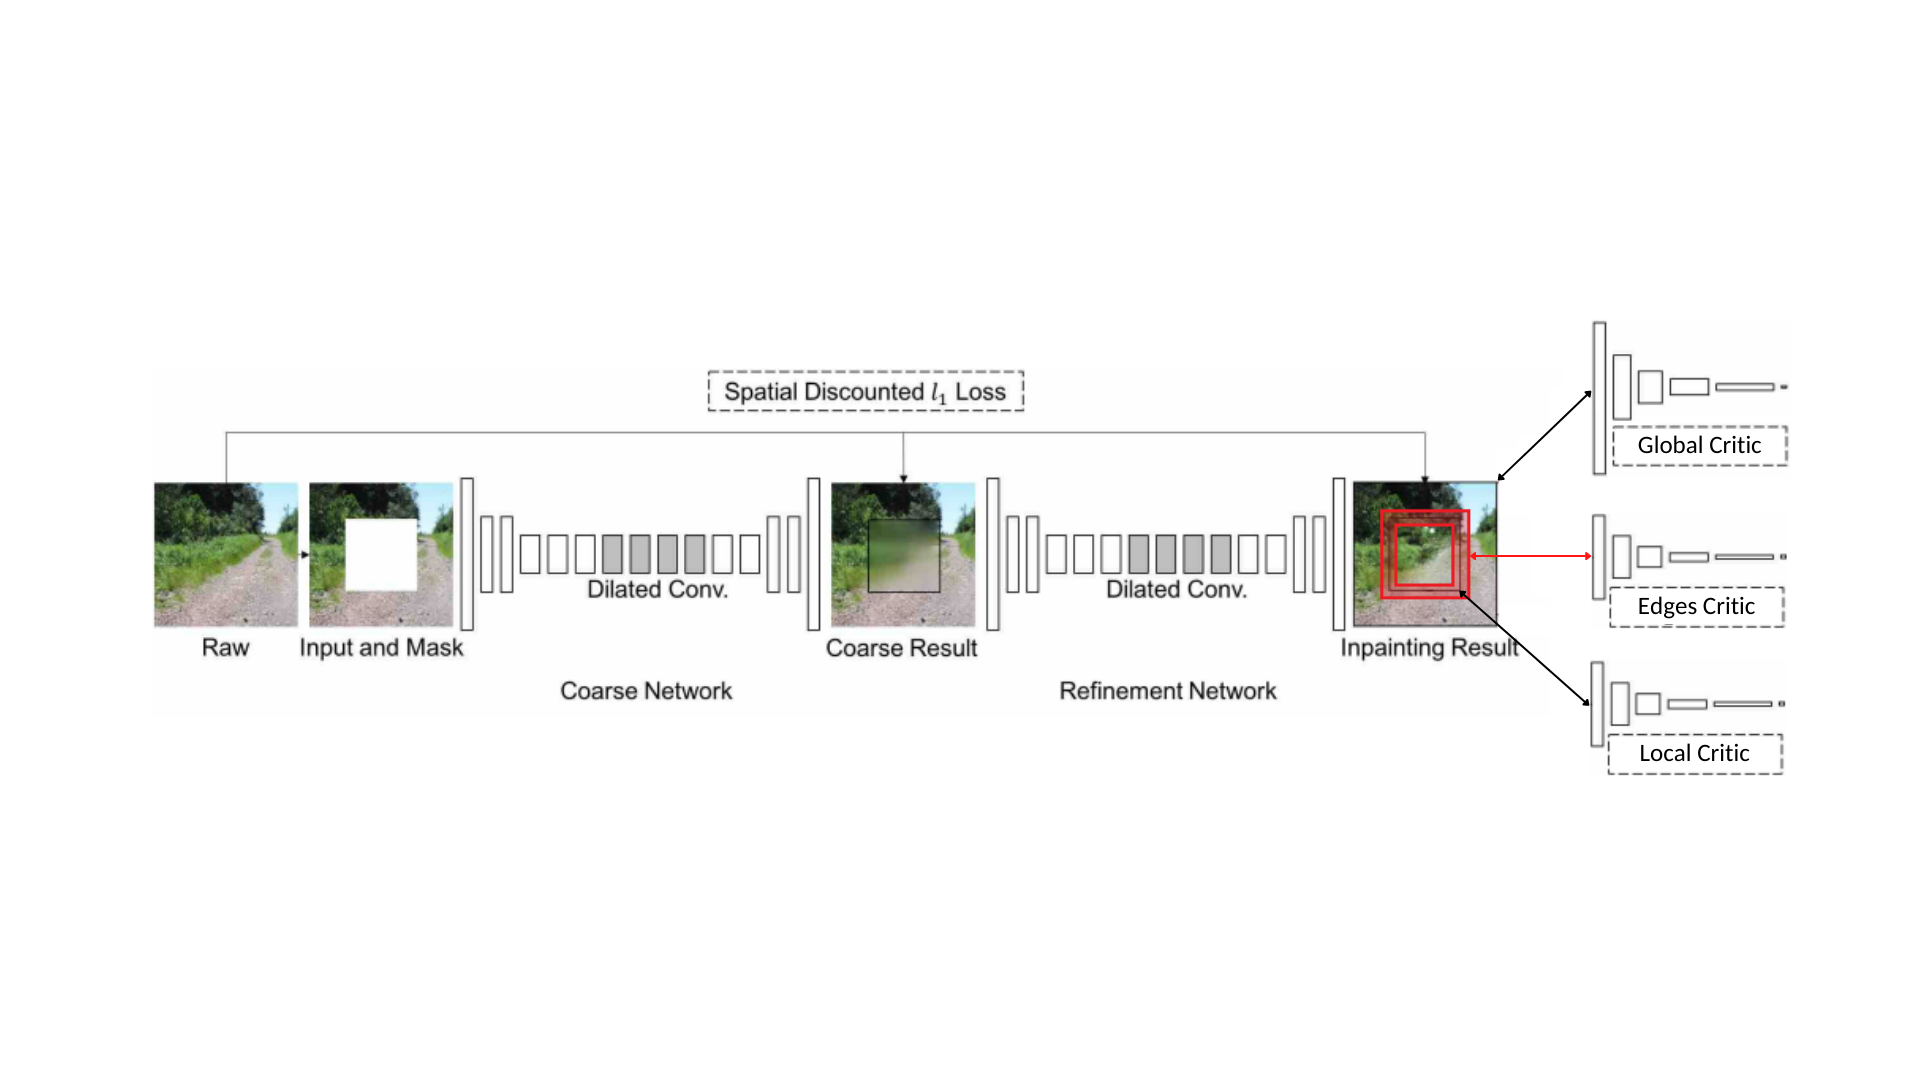
\includegraphics[width=0.95\linewidth]{documentation/img/new_arch.png}
    \end{figure}

\section{Training, testing and validation}
\label{section:training}
We have trained both the baseline and our modified model from scratch, so we can do a comparison.

\section{Results and conclusions}
\label{section:results}
You can see some examples bellow. Every time it is from the left, to the right the original input image, baseline model output, our new improved model output.
\begin{figure}
    \centering
    \begin{minipage}{.3\textwidth}
      \centering
      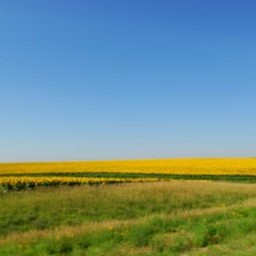
\includegraphics[width=.95\linewidth]{documentation/img/corny_field.jpg}
    \end{minipage}%
    \begin{minipage}{.3\textwidth}
      \centering
      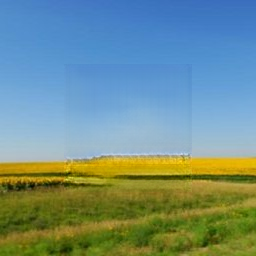
\includegraphics[width=.95\linewidth]{documentation/img/corny_field_out_45k.png}
    \end{minipage}
    \begin{minipage}{.3\textwidth}
      \centering
      \includegraphics[width=.95\linewidth]{}
    \end{minipage}
\end{figure}

\begin{figure}
    \centering
    \begin{minipage}{.3\textwidth}
      \centering
      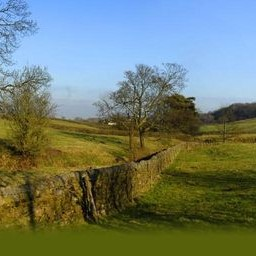
\includegraphics[width=.95\linewidth]{documentation/img/hayfield.jpg}
    \end{minipage}%
    \begin{minipage}{.3\textwidth}
      \centering
      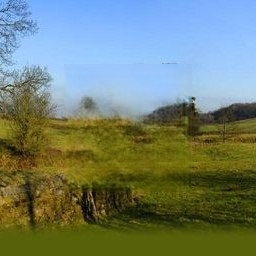
\includegraphics[width=.95\linewidth]{documentation/img/hayfield_out_45k.png}
    \end{minipage}
    \begin{minipage}{.3\textwidth}
      \centering
      \includegraphics[width=.95\linewidth]{}
    \end{minipage}
\end{figure}

\begin{figure}
    \centering
    \begin{minipage}{.3\textwidth}
      \centering
      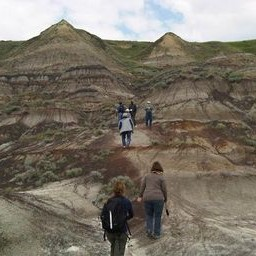
\includegraphics[width=.95\linewidth]{documentation/img/badlands.jpg}
    \end{minipage}%
    \begin{minipage}{.3\textwidth}
      \centering
      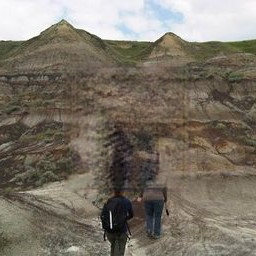
\includegraphics[width=.95\linewidth]{documentation/img/badlands_out_45k.png}
    \end{minipage}
    \begin{minipage}{.3\textwidth}
      \centering
      \includegraphics[width=.95\linewidth]{}
    \end{minipage}
\end{figure}

\begin{figure}
    \centering
    \begin{minipage}{.3\textwidth}
      \centering
      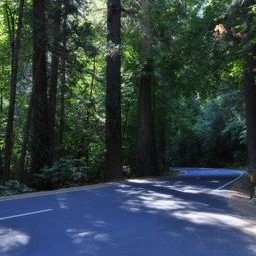
\includegraphics[width=.95\linewidth]{documentation/img/forest_path.jpg}
    \end{minipage}%
    \begin{minipage}{.3\textwidth}
      \centering
      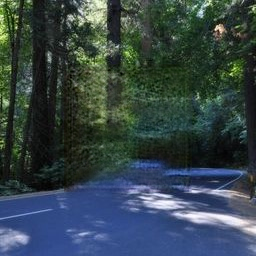
\includegraphics[width=.95\linewidth]{documentation/img/forest_path_out_45k.png}
    \end{minipage}
    \begin{minipage}{.3\textwidth}
      \centering
      \includegraphics[width=.95\linewidth]{}
    \end{minipage}
\end{figure}

\end{document}
